\begin{frame}{An Intelligent Runtime System for Clusters of SMPs}{}
\begin{columns}
\begin{column}{0.5\columnwidth}
  \begin{itemize}
 \small \item \small An adaptive runtime system like Charm++ intelligently balances computational work periodically.
  \item \small Two issues exist when using a basic Charm++ scheduling scheme.
    \begin{enumerate}
    \small \item \small Challenge of the cost of over-decomposition.
    \item \small Challenge and opportunity to exploit multi-core nodes to mitigate imbalance.
    \end{enumerate}
    \item We can address both challenges by:
    \begin{enumerate}
    \small \item \small Having Charm++'s load balancer assign Charm++ objects, i.e., chares, to nodes.% (instead of cores).  
    \item \small Using loop parallelism to distribute work within a node.
    \end{enumerate}
  \end{itemize} 
\end{column}

\begin{column}{0.5\columnwidth}
  \begin{figure}[ht!]
    \begin{center}
      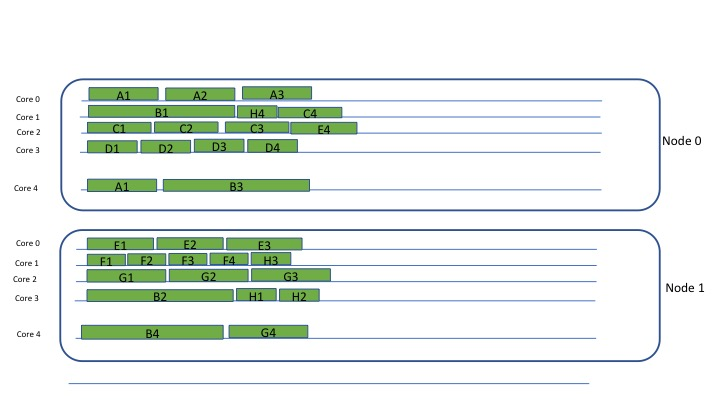
\includegraphics[width=0.75\columnwidth]{./images/CharmLdbWithLoop-manyChares}\\
      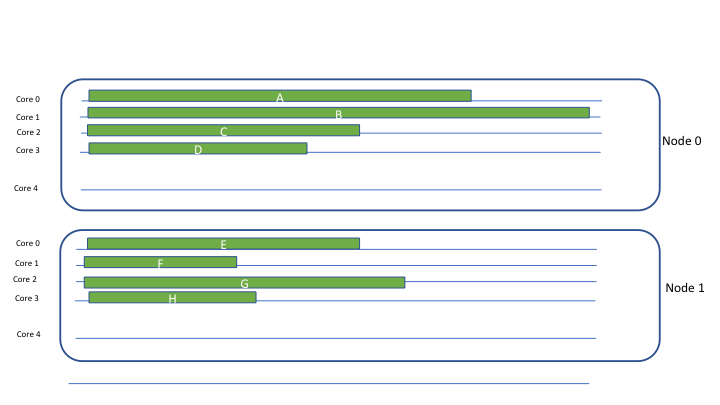
\includegraphics[width=0.75\columnwidth]{./images/CharmLdbWithLoop-fewChares}
      \label{fig:charmcklooptimeline}
    \end{center}
    \caption{\label{fig:charmcklooptimeline}\small Timelines using Charm++-only for default (left) and a mode where the number of chares per node\\ is reduced (right). }
    %Each green rectangle corresponds to execution of a Charm++ object on a core.            
  \end{figure}
\end{column}
\end{columns}
\end{frame}

\begin{frame}{Using Existing Intelligent Strategies for Internode Load Balancing}
\begin{columns}
\begin{column}{0.5\textwidth}
\begin{itemize}
\small \item \small The loop parallelism must handle dynamic imbalances while preserving locality.
\item \small The mixed static/dynamic scheduling previously developed is a promising scheduling strategy for this purpose.
\item \small A solution using only within-node loop scheduling won't handle inter-node load balance that's significant in many applications.
\end{itemize}
{\small $\rightarrow$ Need to modify load balancer so that it uses loop scheduling and is adjusted to reduce overhead of load balancing.}
\end{column} 

\begin{column}{0.5\textwidth}
\begin{figure}[ht!] \label{fig:charmBeforeAndAfterLdBCkLoop}
  \begin{center}
    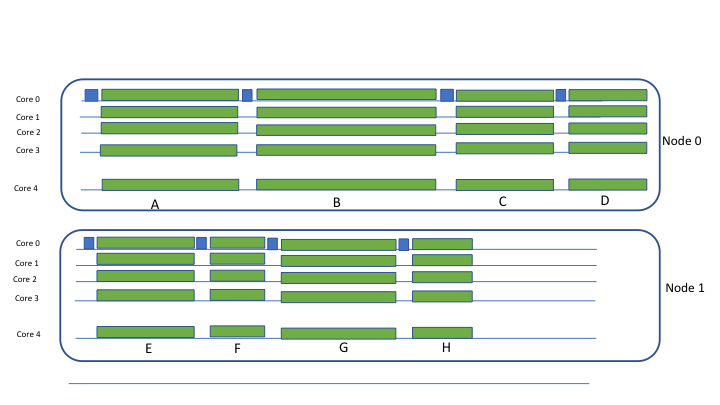
\includegraphics[width=.8\columnwidth]{images/charmLdbWithLoopwCharmonly-unbalanced}\\
    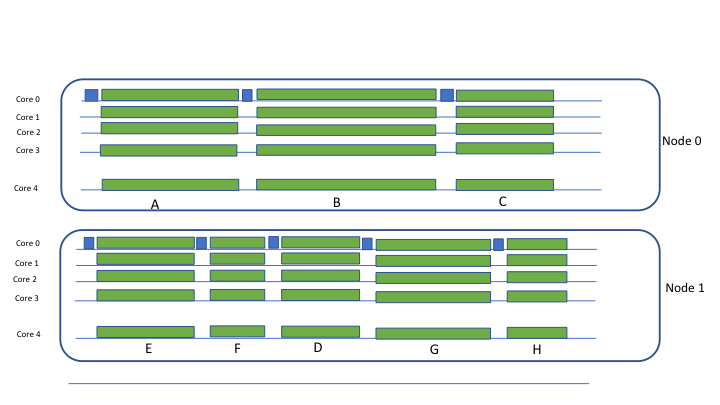
\includegraphics[width=.8\columnwidth]{images/charmLdbWithLoopwCharmonly-balanced}
  \end{center}
  \caption{\label{fig:charmBeforeAndAfterLdBCkLoop} \small Timelines for execution of a code without (left) and with (right) Charm++ load balancing.}
  %\\ A green rectangle on a non-zero core on a node corresponds to loop iterations spawned from core 0. 
\end{figure}
\end{column}
\end{columns}
\end{frame}

\begin{frame}{Key Idea of Our Solution}
\begin{columns}
\begin{column}{0.5\columnwidth}
\begin{enumerate}
 \item Modify Charm++ RTS to assign chares to core 0 of each node only.
 \item Reduce the number of chares per PE.
 \item Adjust parameters of within-node loop scheduler,e.g., vary
  static fraction, based on parameters of Charm++. 
\item Tune Charm++ RTS parameters to work with adjustments of within-node loop scheduling.
\end{enumerate}
\end{column}
\begin{column}{0.5\columnwidth}
  \begin{figure}
    \label{fig:statDynSched}
    \begin{center}
      \subfloat[\tiny Static Scheduling.]{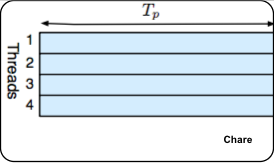
\includegraphics[width=.20\columnwidth]{./images/threadedCompRegion-static-withChare}}\hspace*{0.1in}
               \subfloat[\tiny Dynamic Scheduling.] {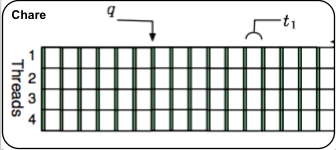
\includegraphics[width=.27\columnwidth]{./images/threadedCompRegion-dynamic-withChare}}\hspace*{0.1in}
                        \subfloat[\tiny Mixed Scheduling] 
 {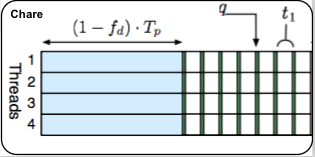
\includegraphics[width=.24\columnwidth]{images/threadedCompRegion-hybrid-withChare}}
    \end{center}
    \caption{\label{fig:statDynSched} \tiny Mixed static/dynamic scheduling within a chare, i.e., a
      Charm++ object.}
  \end{figure}
\end{column}
\end{columns}
\end{frame}

\begin{frame}{Baseline Results and Analysis}{Existence of Within-node Load Imbalance through Heat Maps}
\begin{figure}[ht!]
\begin{center}
{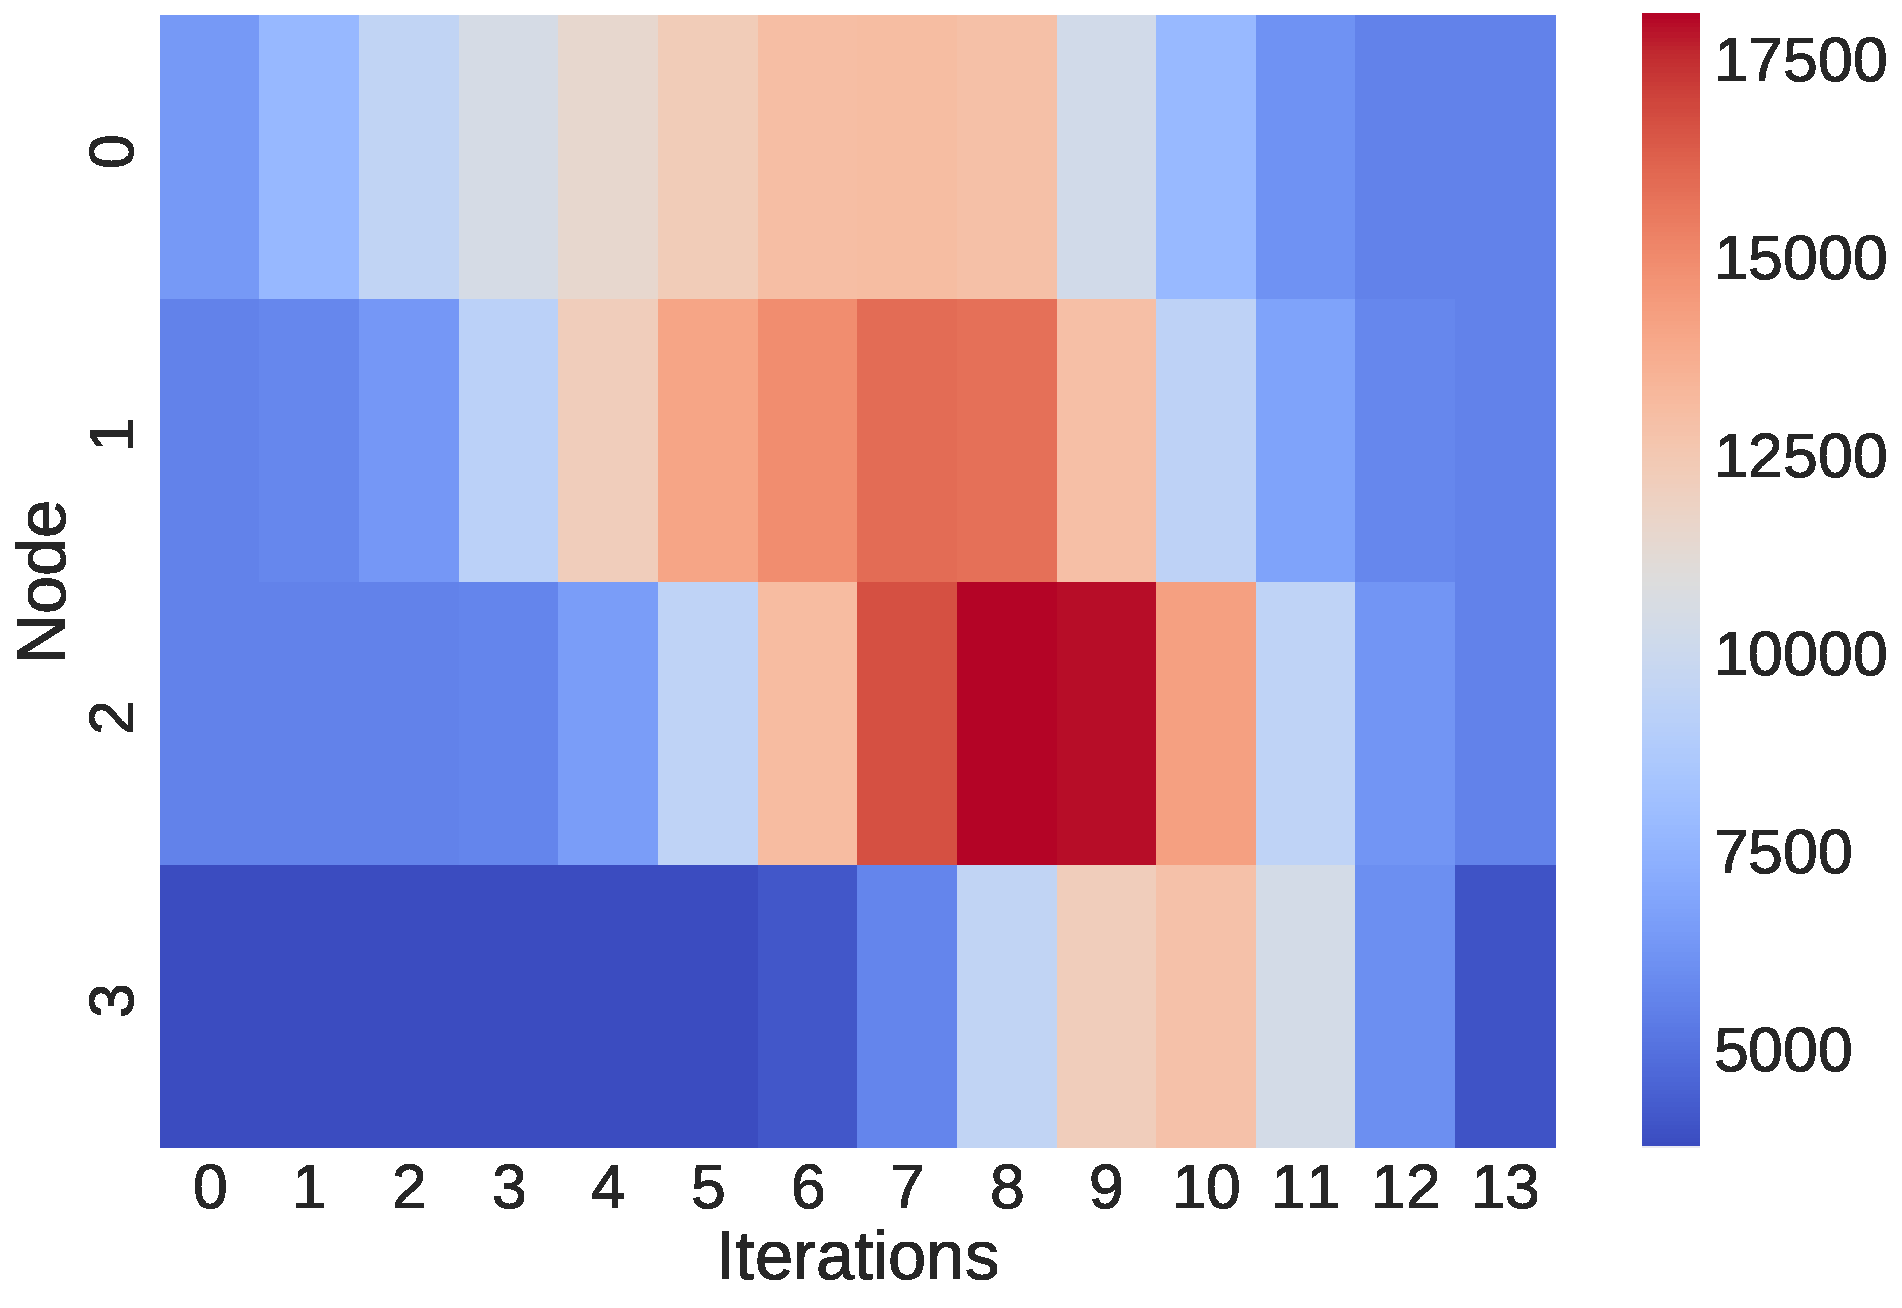
\includegraphics[width=.25\columnwidth]{images/nolb_node_load_with_iter}}
{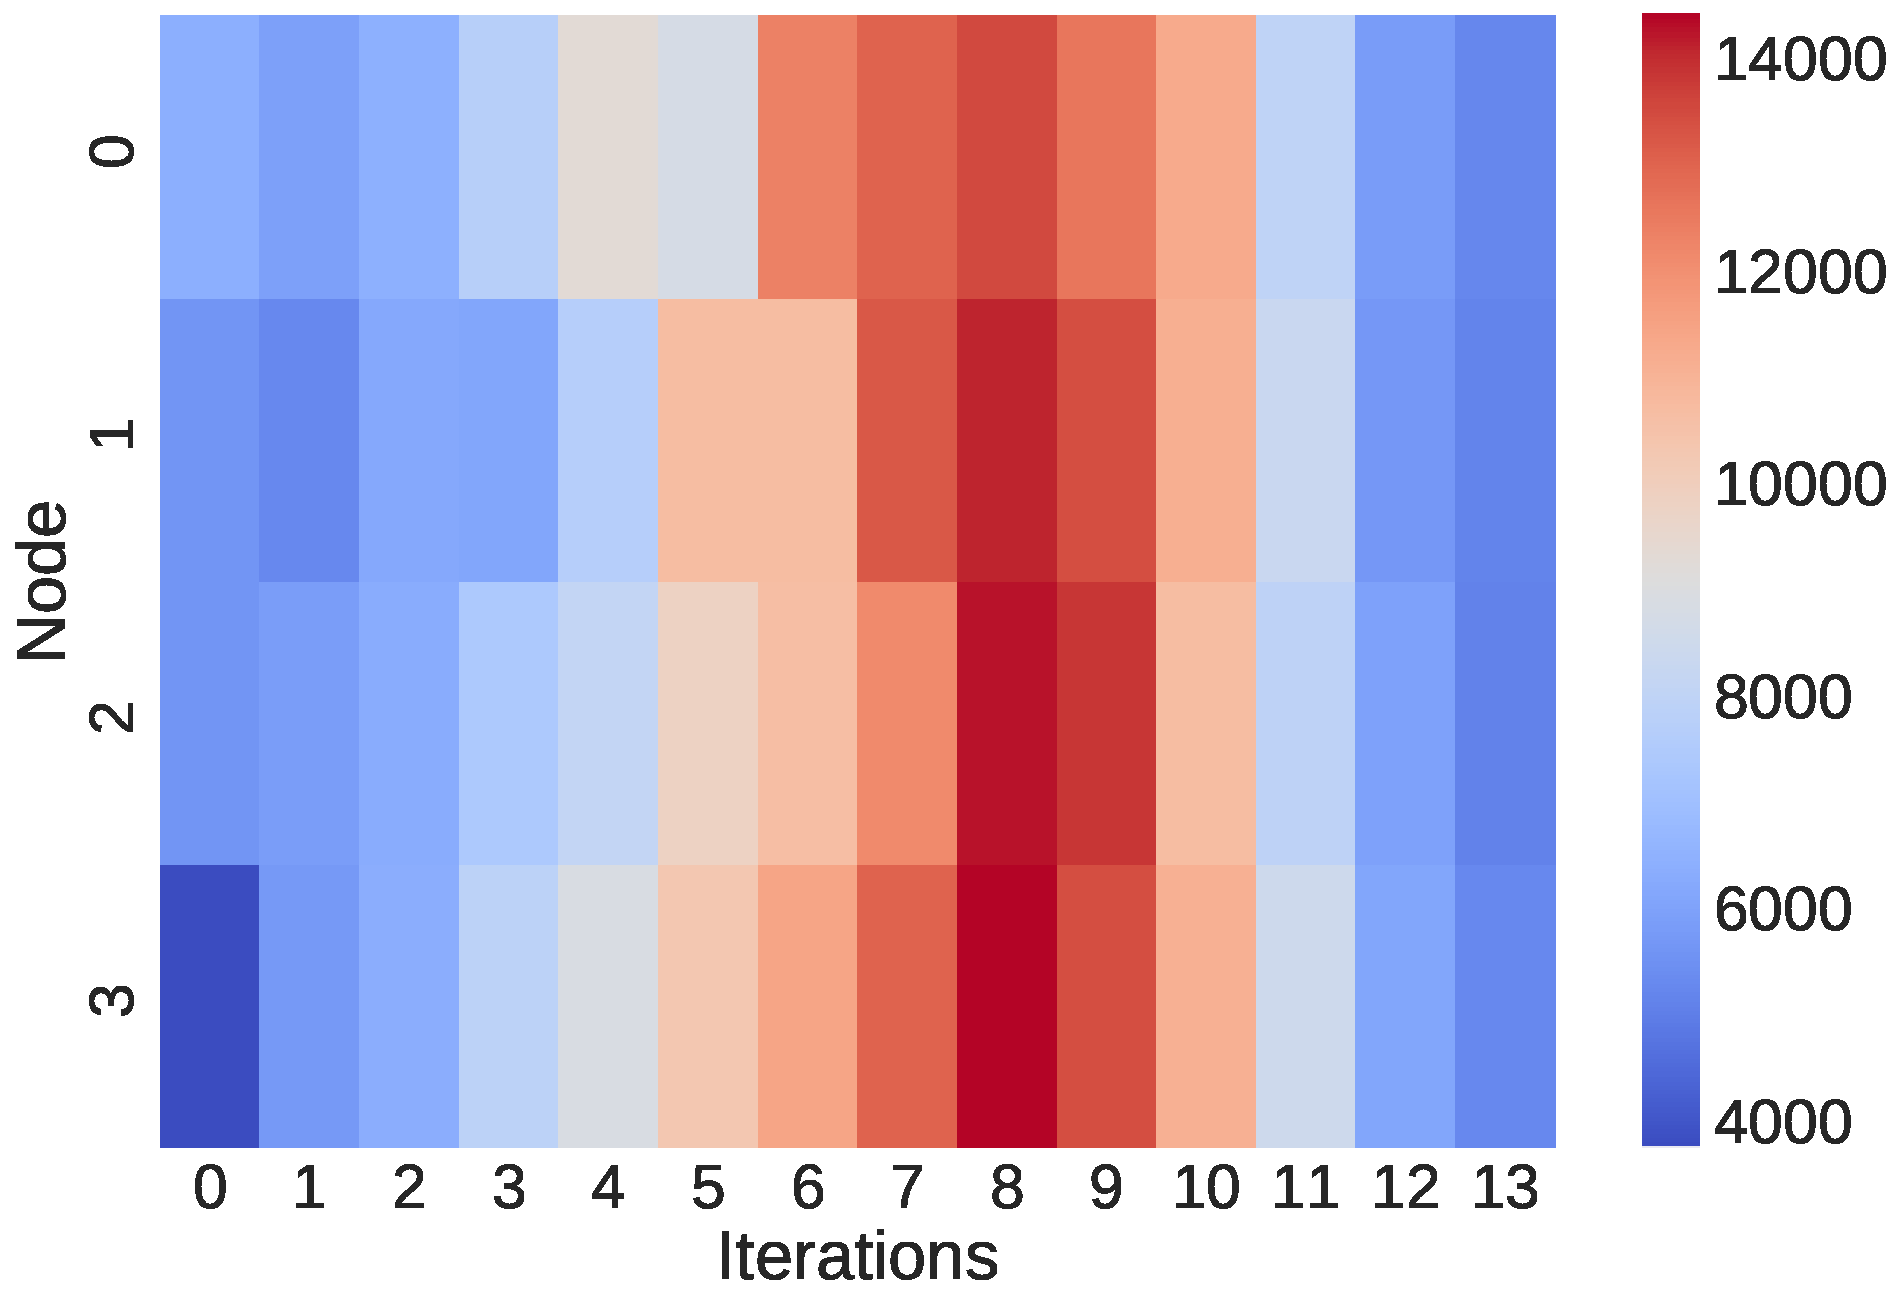
\includegraphics[width=0.25\columnwidth]{plots/greedylb_node_load_with_iter__2_.pdf}}\\
{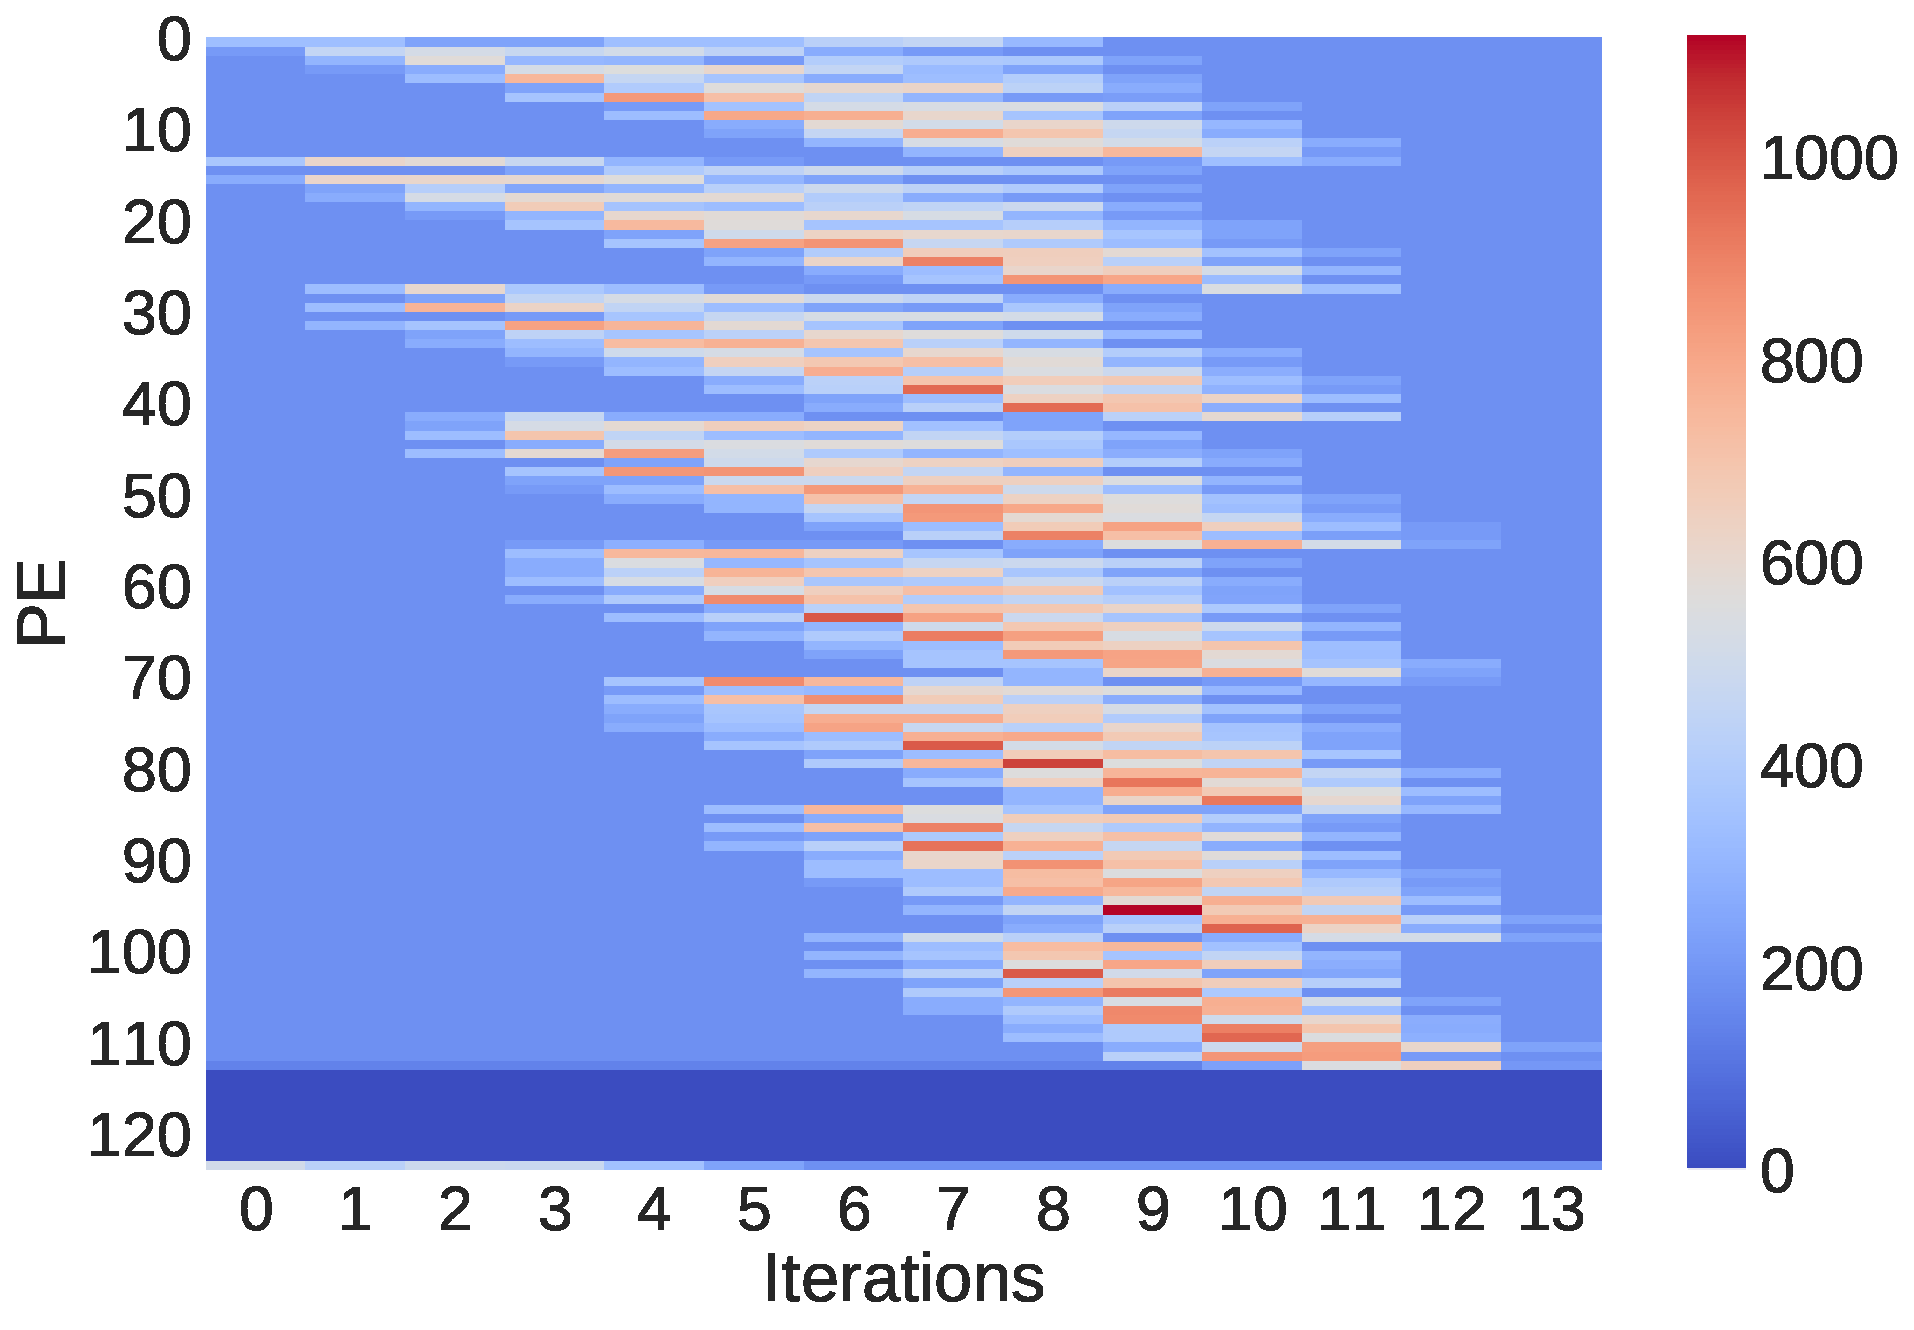
\includegraphics[width=0.25\columnwidth]{images/nolb_pe_load_with_iter}}
{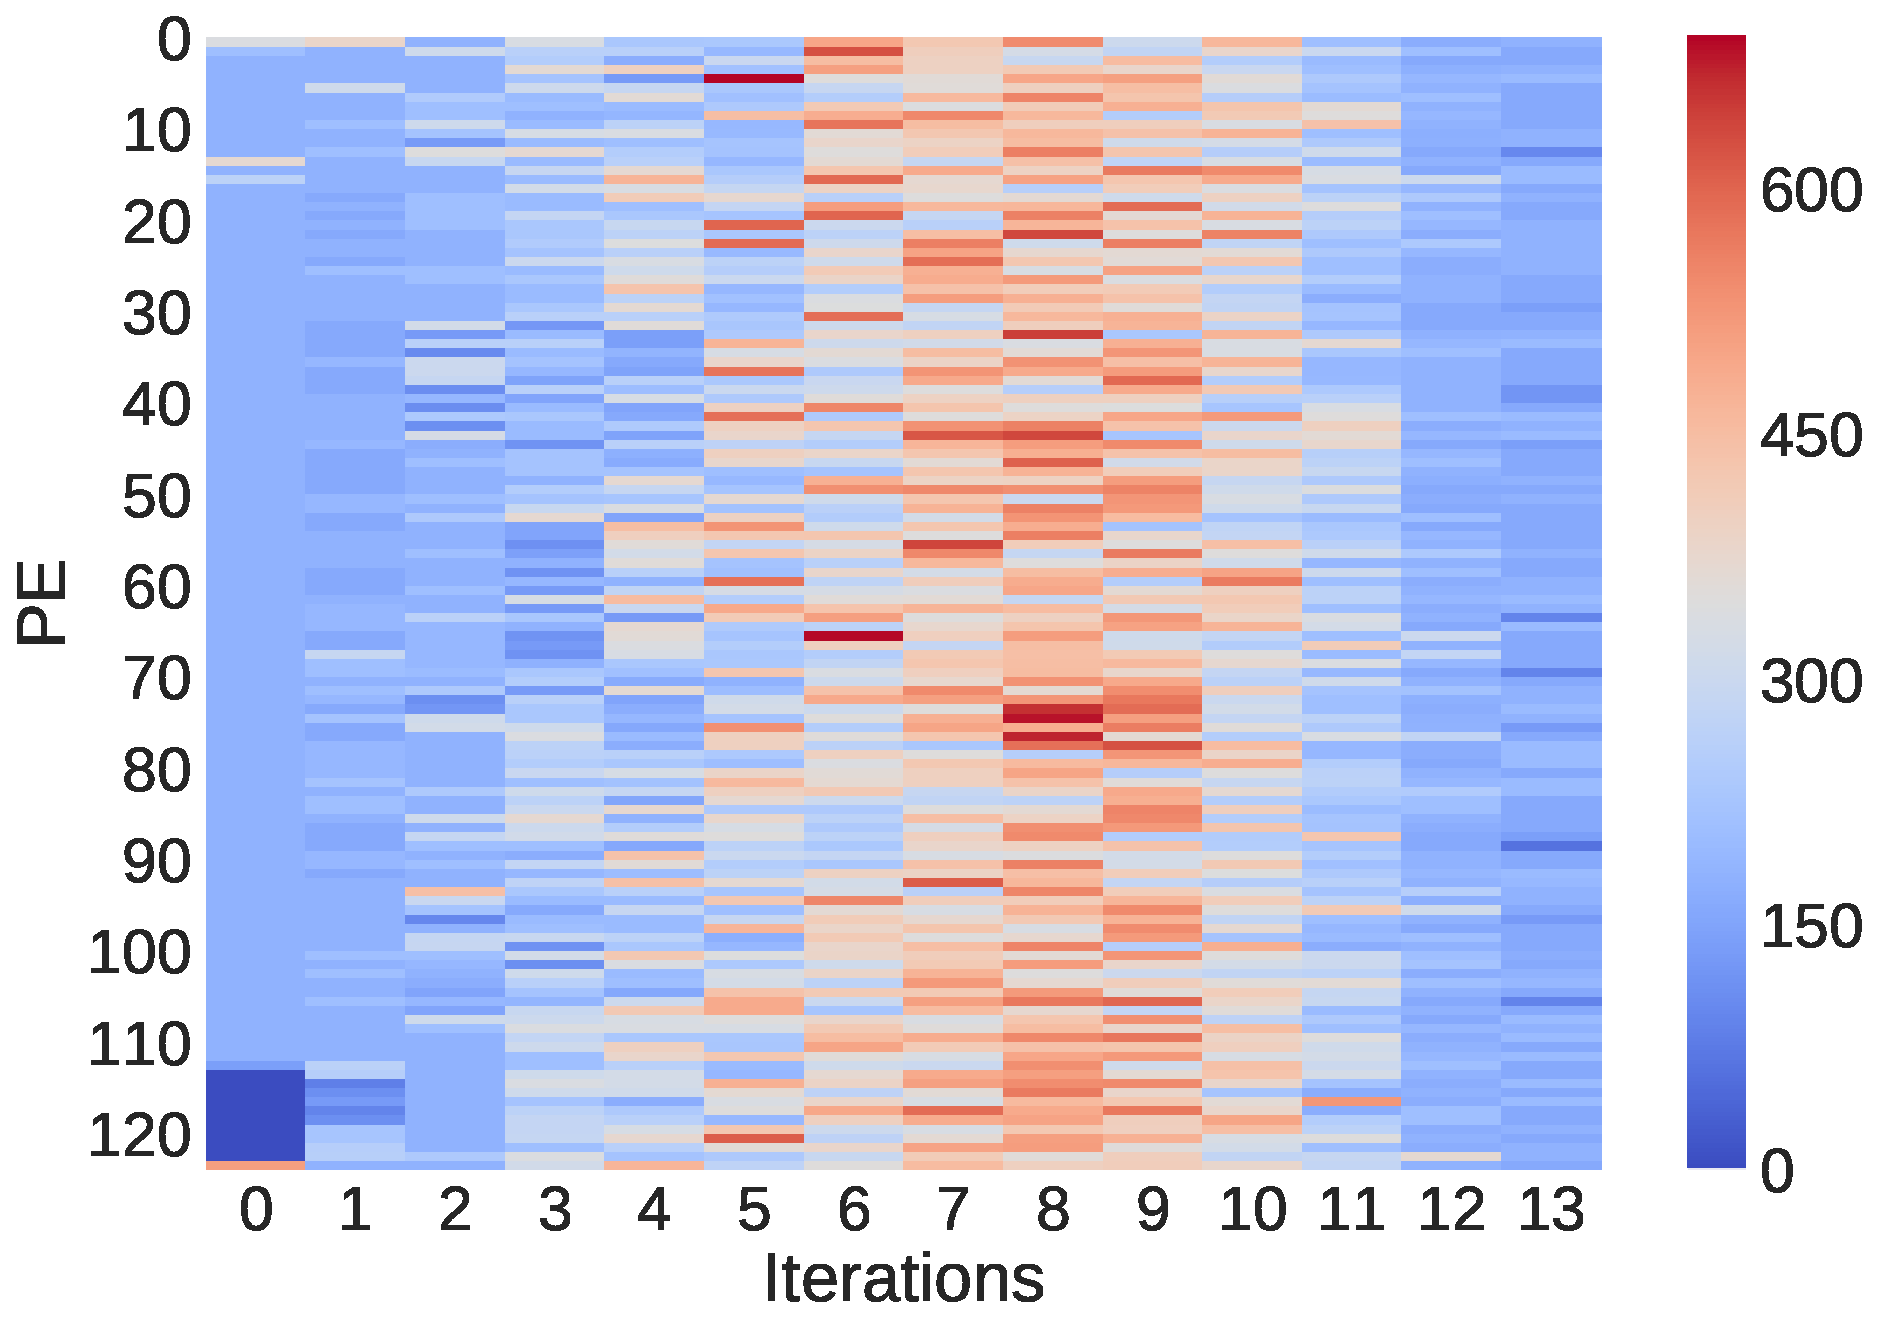
\includegraphics[width=0.25\columnwidth]{plots/greedylb_pe_load_with_iter}}
\end{center}
\caption{\label{fig:motexample2} \footnotesize Load imbalances across nodes (left) and across cores (right) when the greedy load balancing strategy is used.}
\end{figure}
\begin{itemize}
\tiny \item \tiny Using no load balancing, node 2 is heavily overloaded for iterations 8 and 9. Hence, we need load balancing to distribute the load across nodes.
\item \tiny Inter-node load balancing using GreedyLB balances load across nodes well.
\item \tiny Balancing load across nodes using GreedyLB still leaves load imbalance in the cores within a node.
\end{itemize}
\end{frame}

\begin{frame}{Additional Baseline Results}
\begin{figure}
 \label{fig:addbr}
    \centering
  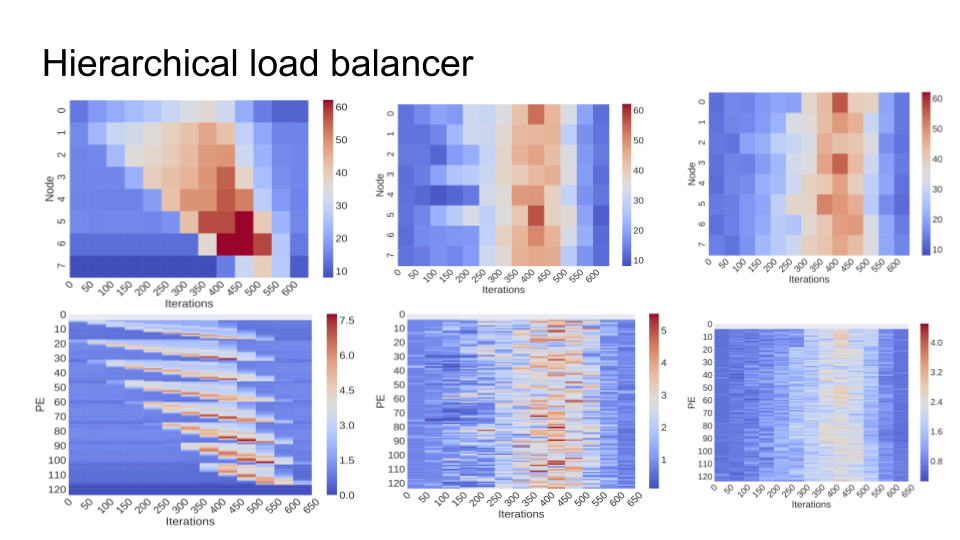
\includegraphics[scale=0.3]{plots/additionalBaselineResults.png}
  \caption{\label{fig:addbr}Baseline Results for Lassen Using Charm++ + OpenMP implementation shown in the middle.} 
\end{figure}
\end{frame}

\begin{frame}{Proposed Set of Techniques}
  \begin{enumerate}
  \item We decide on the combinations of advanced loop scheduling and advanced load balancing strategies to use. 
  \item We either experimentally tune or use an automated technique to adjust parameters of load balancing and loop scheduler together to improve performance of application. 
  \item We then consider advanced load balancing and loop scheduling strategies that can help for the combined load balancing and loop scheduling technique.
  \end{enumerate} 
\end{frame}

\begin{frame}{Performance Model for Load Balancing and Loop Scheduling}
            % first row is the table of parameters                          
            \begin{table}[h!t]
              \centering
              \label{tab:pmta}
              \begin{tabular}{|l|l|}
                \hline
                \tiny$t_1$    & \tiny Duration of a loop iteration\\ %iteration on one core \\
                \hline
                \tiny$T_p$    & \begin{tabular}[c]{@{}l@{}}\tiny Total execution time of a threaded computation region\vspace*{-0.3in} \\ \tiny consisting of $N$ loop iterations on $p$ cores\end{tabular} \\ \hline
                  %             \tiny$q$      & \tiny Scheduler's dequeue overhead of a loop iteration                                                                 \\ \hline  
                  %             \tiny$d$  & \tiny Time for executing an iteration dynamically 
                  \\ \hline
                  \tiny$\delta$ & \tiny Expected cost of load imbalance on a node to the application                                         \\ \hline
                  \tiny$load_i$ & \tiny Load on the $i^{th}$ core of a node on an arbitrary timestep                             \\ \hline
              \end{tabular}
              \caption{\label{tab:pmta} \tiny Terms in implementation}
            \end{table}
\end{frame} 

\begin{frame} 

\begin{itemize} 
\item We refer to this scheduling strategy as \emph{adaptive loop scheduling} and use a parametrized version of it to schedule loop iterations of a chare to cores. 
\item The best-performing collection of scheduler parameter values is the best-performing one, on average, for each chare. An optimal collection of scheduler parameter values, in isolation, isn't necessarily the best-performing, given an arbitrary collection of parameter values for the load balancer. 
\item Thus, our technique is to search for the collection of parameter values for the scheduler together with those for the load balancer that obtains best performance.
\end{itemize} 

\end{frame} 


\begin{frame}{Technique} 

\begin{columns}
\begin{column}{0.5\columnwidth}
{\scriptsize \underline{\textbf{Scheduling Strategies}}}
 \begin{itemize}
 \tiny \item \tiny Mixed static/dynamic
 \item \tiny Weighted dynamic
 \item \tiny Staggered
 \end{itemize}
{\scriptsize \underline{\textbf{Load Balancing Strategies}}}\\
\begin{itemize}
\tiny \item \tiny Periodic
\item \tiny Hierarchical
\end{itemize}
\end{column}


\begin{column}{0.5\columnwidth} 
{\scriptsize \underline{\textbf{Parameters of Scheduler}}}\\
\begin{enumerate}
\tiny \item \tiny Static fraction.
     \item \tiny Chunk size.
     \item \tiny Distribution of chunk sizes in queue.
     \item \tiny Cores per steal queue.
\end{enumerate}
{\scriptsize \underline{\textbf{Parameters of Load Balancer}}}\\
\begin{enumerate}
 \tiny \item \tiny Chares per PE.
 \item \tiny Frequency of load balancing step.
           % TODO: word the bullet above better
\end{enumerate}  
\end{column}
\end{columns}
         \begin{figure}[ht!]
           \label{fig:charm++locopthybsched}
           \begin{center}
             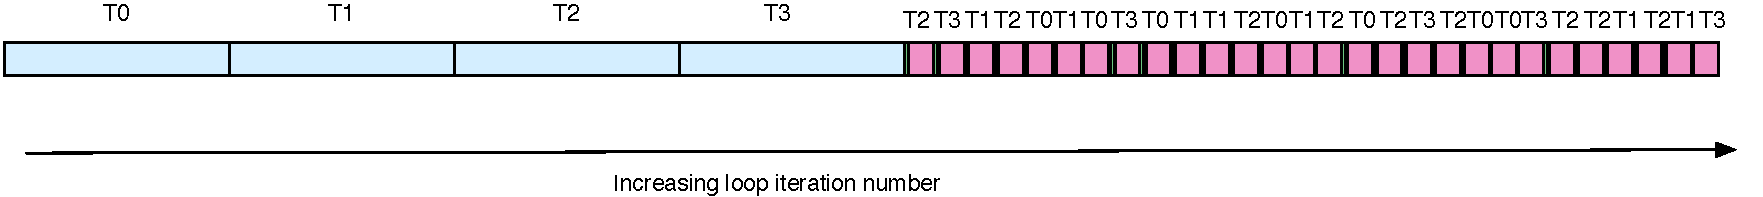
\includegraphics[scale=0.2]{./images/sdIncrIters}\\
             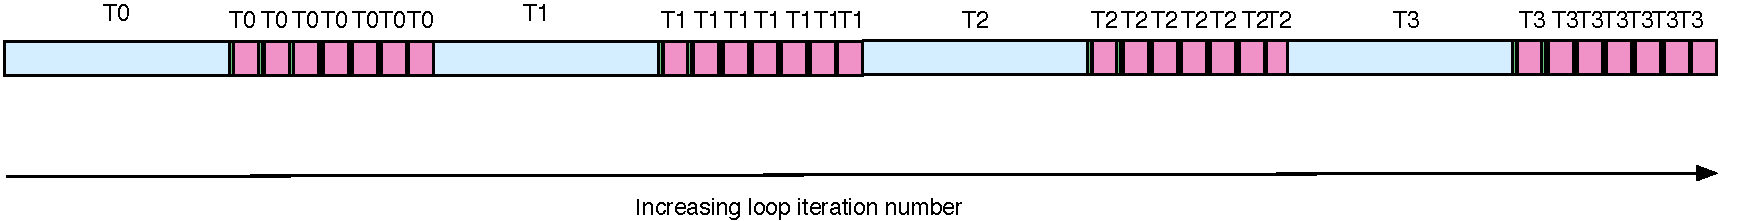
\includegraphics[scale=0.2]{./images/sdsIncrIters}
           \end{center}
           \vspace*{-0.1in}
           \caption{\label{fig:charm++locopthybsched} \tiny Mixed static/dynamic scheduling using an optimization of iteration staggering}
         \end{figure} 
         
         {\scriptsize \underline{\textbf{Methodology for Tuning Parameters}}}
         \begin{itemize}
               \tiny \item \tiny The parameters of the load balancer and of the scheduler can't be tuned independently.
             \item \tiny We tune the parameters of the scheduler and load balancer together.
         \end{itemize} 
   \end{frame} 
   
\begin{frame}{Advanced Load Balancing Techniques} 
\begin{itemize}
\item A hierarchical strategy for load balancing
\begin{itemize}
\item Frequent intra-node load balancing.
\item Infrequent inter-node load balancing.
\end{itemize}
\item Inter-node load balancing strategy would distribute work load taking into account
\begin{itemize}
\item Topology aware
\item GPU + CPU hybrid architecture
\end{itemize}
\item Use machine learning techniques to decide the most suitable strategy to use.
\end{itemize}
\end{frame} 

   
   
\begin{frame}{Loop Scheduling Techniques}
The following loop scheduling techniques will be beneficial in the
context of this work.
\begin{itemize}
\item Tapering:
\begin{itemize}
\item Useful for workloads with irregular load imbalances
\end{itemize}
\item Weighted dynamic.
\begin{itemize}
\item Helpful when certain cores within a node are slow.
\item Uses ideas of measurement-based load balancing
\end{itemize}
\item Tuning task gain size distribution.
\begin{itemize}
\item Helpful when certain cores have irregular load imbalances
\item Can adjust scheduler parameters based on across-node load balancing parameters.
\end{itemize}
\item Locality-aware constrained loop scheduling.
\end{itemize}
\end{frame}

%\bbi\item Bullet 1\onslide<2->{\item Bullet %2}\onslide<3->{\item Bullet 3}\onslide<4->{\item %Bullet 4}\ei

\begin{frame}{Implementation}{Overview of Software Architecture}
\begin{figure}[ht!]
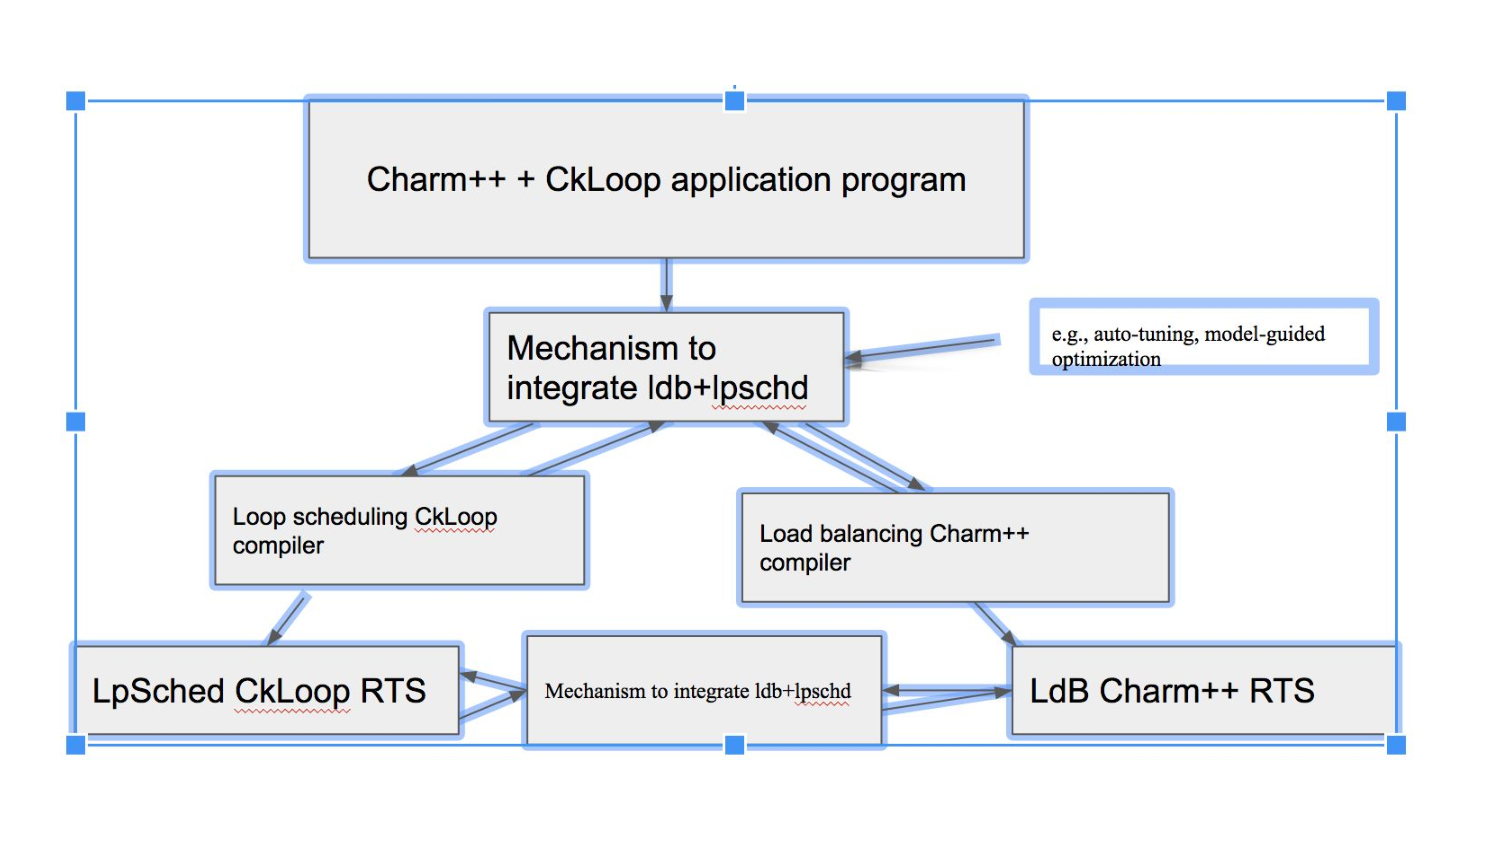
\includegraphics[scale=0.4]{./images/lslb_softwarediagram}
\caption{Diagram of Software Infrastructure for Load Balancing and Loop Scheduling Technique}
\end{figure}
\end{frame}

%\noindent {\bf Using the Modified Charm++ RTS}
\section{Modified Charm++ RTS}

\begin{frame}{Usage of Library}
%\sloppy
%\subsubsection{Usage of Library}
%in the lines of code.
\vspace*{-0.1in}
\begin{figure}[h!t]
%\label{code:dotpcharmckhyb}
%\begin{center}
%\lstinputlisting{./listings/dotpcharmckhyb-short.cc}
%\vspace*{-.2in}
%\caption{{\label{code:dotpcharmckhyb}User code for dot product implemented in Charm++ with {\tt CkParLoop()}.}}
%\end{center}

    \label{code:dotpCharmckhyb}
    \lstinputlisting{./listings/old-dotpcharmckhyb.cc}\hspace*{-1.9in}
    \vspace*{-0.8in}\caption{\label{code:dotPCharmckhyb}{\tiny  \label{code:dotpCharmckhyb} Dot product code's modification using Charm++ with CkLoop.}}
 
\end{figure}

\begin{itemize} 
\tiny  \item \tiny Figure~\ref{code:dotpcharmckhyb}
shows the user code with the adapted CkLoop library using the function {\tt CkParLoop()} for the computational region of the program.
\item \tiny The user creates a kernel for the computation region and replaces the region with a call to {\tt CkParLoop()} having the name of the kernel for the computation region as a parameter to the function.
\item \tiny Here, the user calls the function on thread 0 providing the kernel to be called, the range of iterations of the loop and the number of chunks used in the loop. 
\item \tiny The user specifies a loop history variable that has a field for the static fraction within it. 
\item \tiny The lines of code in the user code with the library is 3\% more than the original user code.
\end{itemize} 
\end{frame} 


\comments{
\begin{frame}{Implementation}{Front-end Code}
     % \vspace*{1.3in} 
     % TODO: make this subtly clear in the poster paper - a reviewer of this poster or a possible subsequent paper of this work may ask, 'why don't you do runtime adjustment of parameters or model-guided optimization?' Answer: model-guided optimization is challenging to do for an n-body simulations because of the difficulty in mathematical formulation of application's computat\
     %ion cost. For runtime adjustment, we don't want to formulate a solution prematurely.  
     % We choose experimental performance tuning to further understand our problem and develop a more sophisticated solution later. 
  \begin{figure}[h!t]
    \label{code:dotpCharmckhyb}
    \lstinputlisting{./listings/old-dotpcharmckhyb.cc}\hspace*{-1.9in}
    \vspace*{-0.8in}\caption{\label{code:dotPCharmckhyb}{\tiny  \label{code:dotpCharmckhyb} Dot product code's modification using Charm++ with CkLoop.}}
  \end{figure}
\end{frame}  
}
%\begin{frame}{Implementation}{Back-end Code Design}
%\end{frame}

\begin{frame}{Implementation of Library}
\begin{itemize}

\small \item \small When {\tt CkParLoop()} is invoked on core 0, our scheduler enqueues a message in every core's queue describing the loop. 
\item \small Each core enqueues its dynamic iterations into its own stealable task queue and then executes its static chunk by calling the user-supplied kernel function. 
\item \small It then executes dynamic tasks from its own stealable queue and then randomly steals from other cores' queues.
\item \small The synchronization for loop termination and handling of reduction variables is also part of the implementation.
\item \small  Charm++'s scheme to allocate chares, i.e., objects, to cores was modified so that objects are initially assigned to core 0 of each node. 
\item \small The dynamic load balancer was modified to measure the loads of objects correctly in presence of the scheduler and to ensure that objects weren't re-assigned to cores other than core 0.
\end{itemize}
\end{frame} 


%\begin{frame}{Implementation of CkLoopHybrid}
%\begin{itemize} 
%\item 
%\item 
%\end{itemize} 
%\end{frame}

\begin{frame}{Experimental Setup}
   \underline{Applications}\\ 
   \begin{enumerate} 
   \item {\bf dot Product:}
   \item  {\bf PIC:} not much load balance.
  \item {\bf Lassen:} Can make modifications to the code easily and will be a good benchmark 
  \item {\bf Barnes Hut}
  \end{enumerate} 
  \underline{Setup of Compiler and Runtime}\\
  \begin{enumerate}
      \item Use default compile time options, i.e., '-O3'
      \item Run with drone mode , i.e., one chare per node. 
  \end{enumerate} 
  \underline{Architectures} \\
  \begin{enumerate}
  \item \textbf{BlueWaters}:
  \item \textbf{Cori}:
  \end{enumerate} 
%  3D stencil with dynamic load imbalance injected: need to simply download from repository and insert CkLoopHybrid in it. 
  % contrary to earlier email discussion that it wouldn’t be worth it. 
\end{frame}


\begin{frame}{Results}
\begin{figure}[ht!]
          \begin{center}
            \subfloat[\tiny Dot Product on 4 nodes of Stampede.]{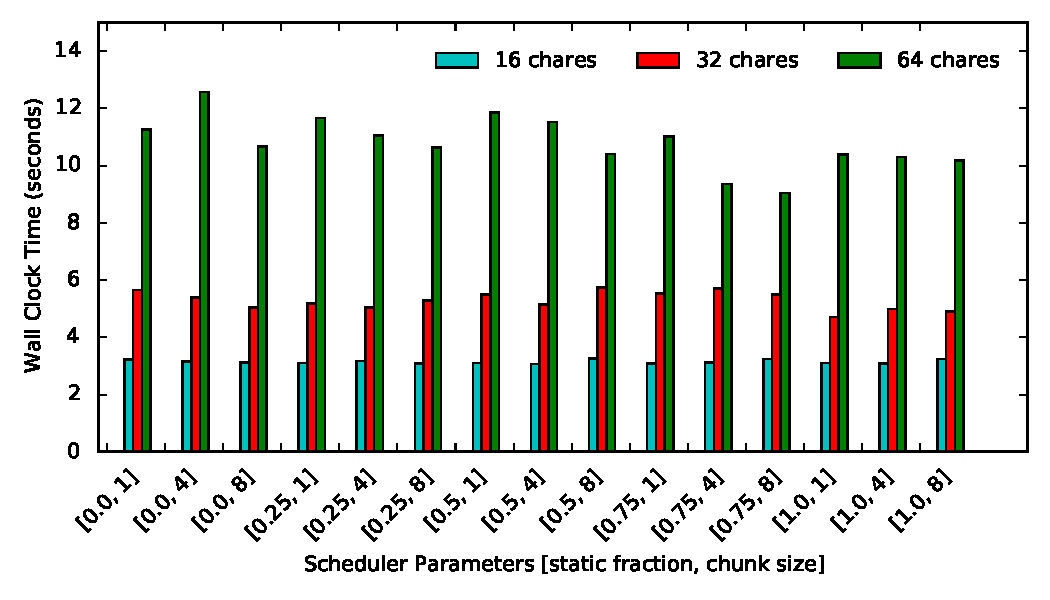
\includegraphics[width=.45\columnwidth]{plots/dotProd-4nodes-bw}} %TODO: replace with dot product results
            \subfloat[\tiny Particle-in-Cell on 4 nodes of Blue Waters.]{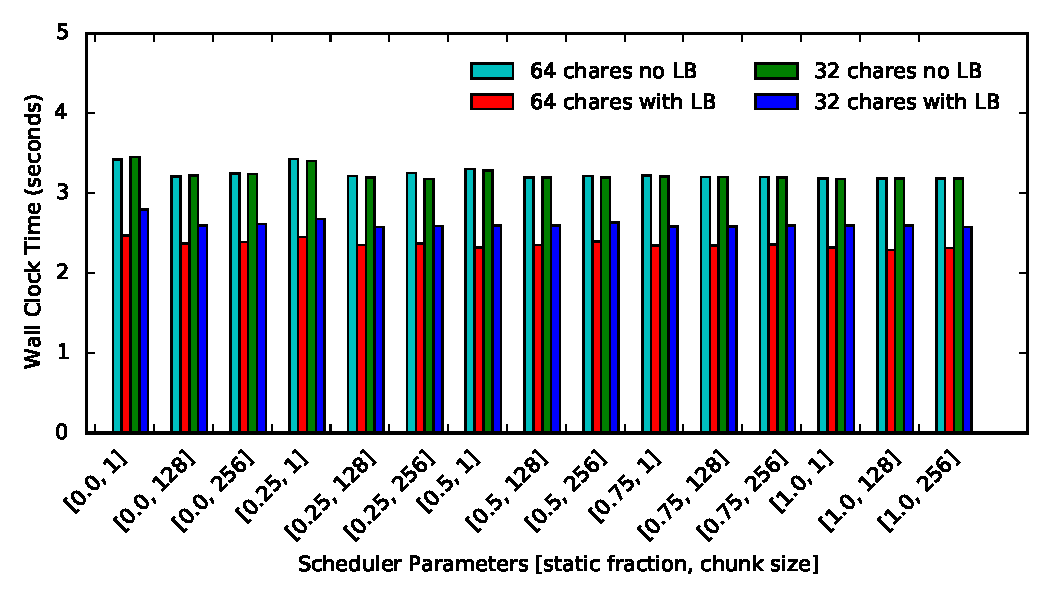
\includegraphics[width=.45\columnwidth]{plots/PIC-4nodes-bw}}
          \end{center}
          \caption{\tiny Execution times of scientific applications on multi-core clusters.}\label{fig:scalability-results-PIC-BW}
        \end{figure}
        
        
%\begin{figure}[ht!]
%\label{fig:resultsLSB}
%  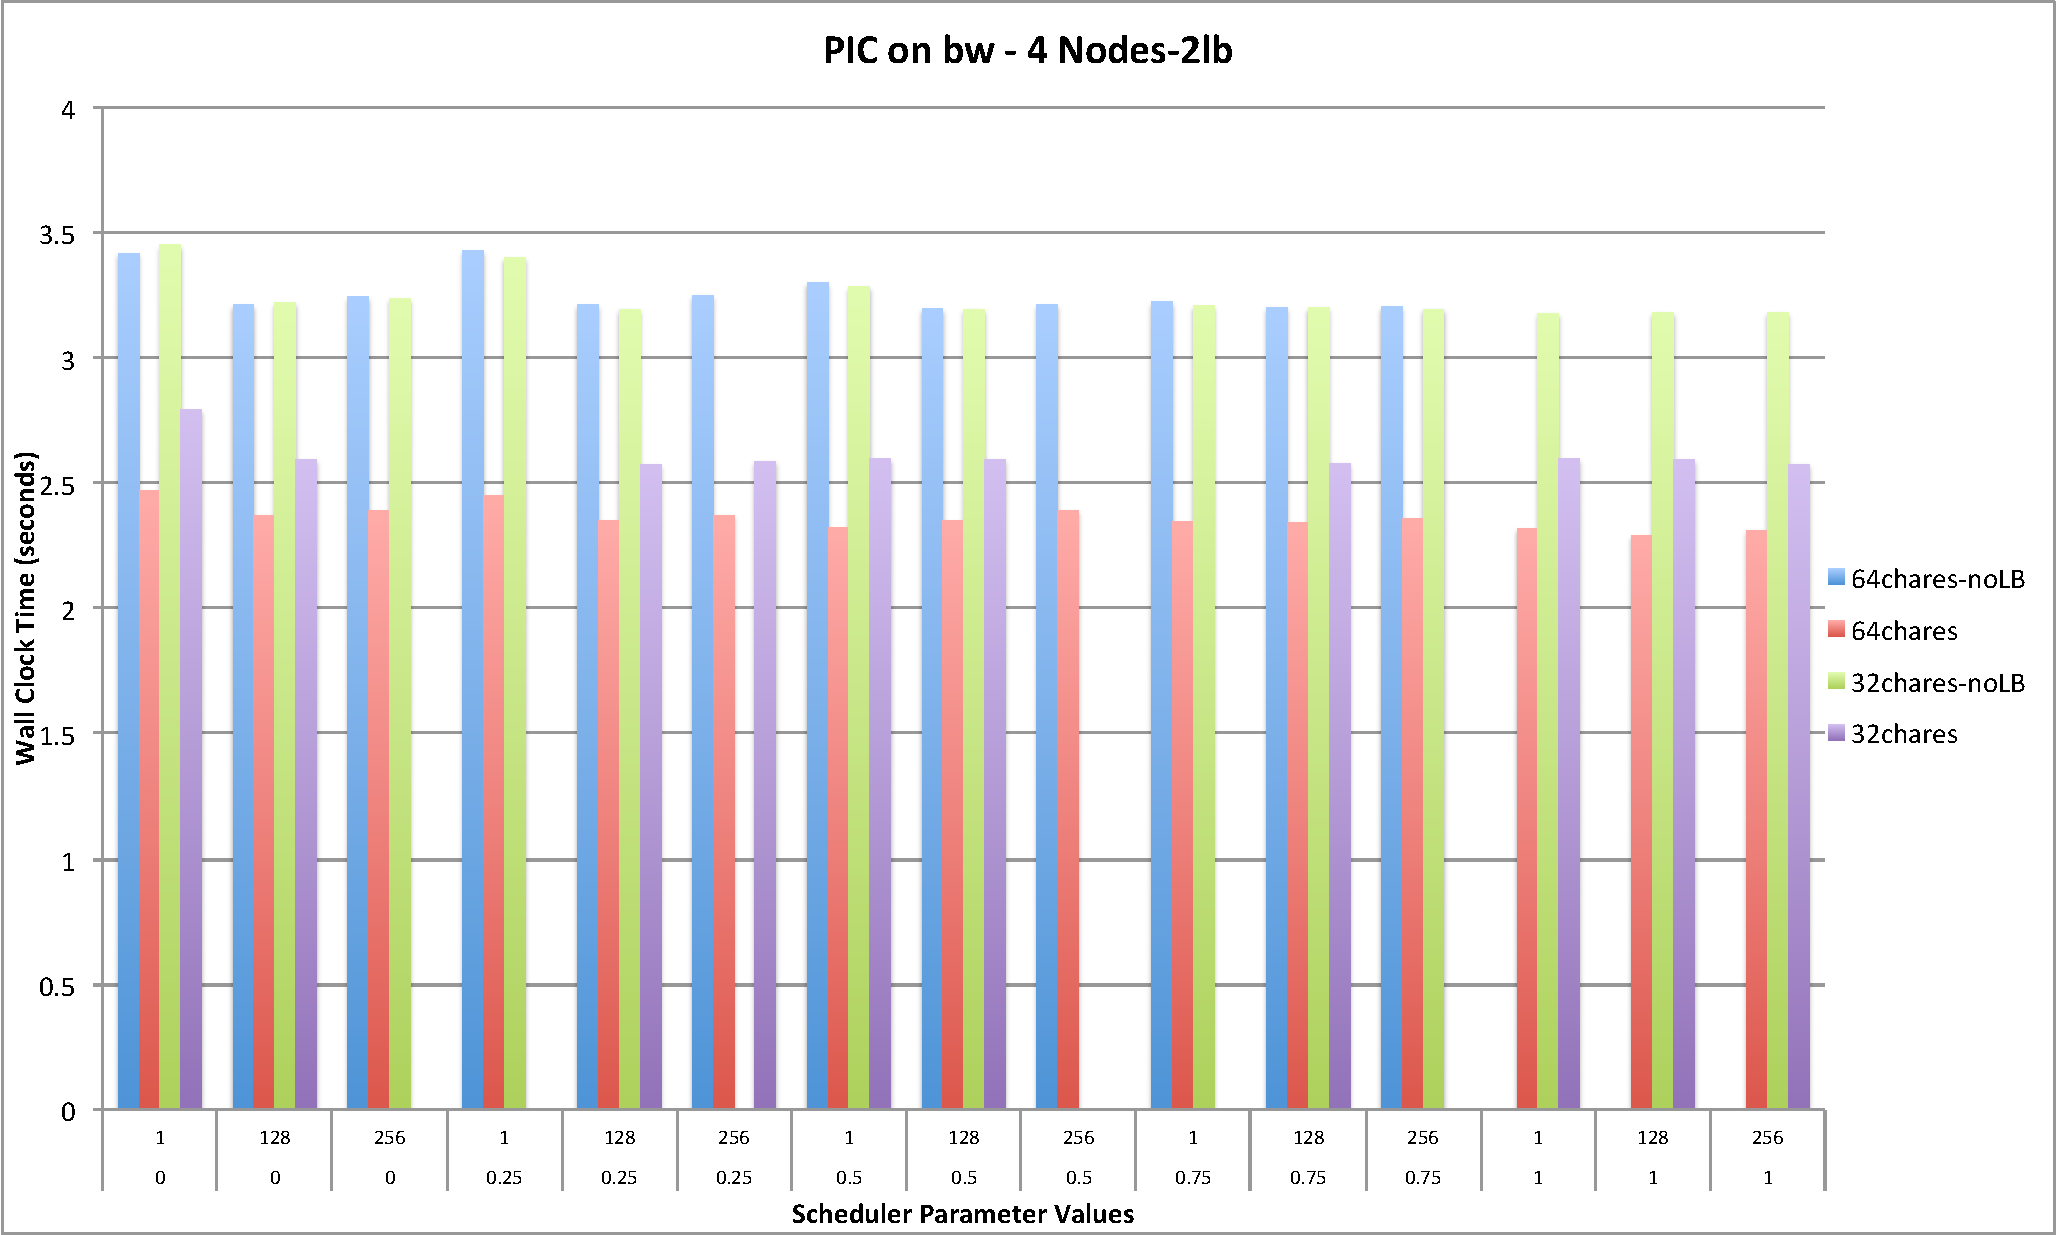
\includegraphics[scale=0.25]{plots/PIC-BW-4nodes-2lb.pdf}
%    \caption{\label{fig:resultsLSB}\small Results of using combined loop scheduling and load balancing approach in a Charm++ + CkLoop program.}
%\end{figure}

\begin{itemize} 
\item \tiny For dot product using 64 chares, a static fraction of 75\% with a chunk size of 8 gives the best performance, showing utility of adaptive loop scheduling.
\item \tiny PIC using modified inter-node load balancing with adaptive loop scheduling is 19.13\% faster than PIC using adaptive scheduling without load balancing.
%\item \tiny The percentage improvement over the original Charm++ + CkParLoop is 17.20\%.
%TODO: Fix the sentence below further to make clear what is going on. 
\item \tiny Synergistic performance improvements using combination of inter-node and intra-node load balancing. 
\end{itemize} 
\end{frame}

\begin{frame}{Related Work} 
\begin{itemize}
    \item Habanero\cite{}: library with support for data locality within node 
    \item MPI+OpenMP\cite{}: basic hybrid parallel programming model.
    \item OmpSS\cite{}: library for extensible loop scheduling schemes.
\end{itemize}
\end{frame}


\begin{frame}[label=lsbconcl]{Conclusion}{Load Balancing and Loop Scheduling}
\begin{enumerate}
\tiny \item \tiny Need sophisticated loop scheduling in Charm++. 
\item \tiny Described a technique and implementation to improve performance of applications. 
\item \tiny Using our technique and implementation, we demonstrate performance improvement \\ of 17.2\%.
\item \tiny For future work, we'll explore other adjustments to parameters of the Charm++ RTS to facilitate for loop scheduling. 
\end{enumerate} 

\end{frame}